%%%%%%%%%%%%%%%%%%%%%%%%%%%%%%%%%%%%%%%%%%%%%%%%%%%%%%%%%%%%%%%%%%%%%%%%%%%%%%%
%  Alocação de computação de inferência na síntese de programas — ARC-AGI-1
%  Template: AAAI Press AuthorKit 2027 (aaai2027.sty)
%
%  ============================================================================
%  COMO ATUALIZAR ESTE ARTIGO QUANDO OS RESULTADOS MUDAREM
%  ============================================================================
%  Todo número do texto, das tabelas e da figura vem de um \newcommand no
%  PAINEL DE RESULTADOS abaixo. Nada é digitado solto no corpo.
%
%   1. Troque os valores no PAINEL. Macros terminadas em "N" são a versão
%      numérica (ponto decimal) lida pela figura; a irmã sem "N" é a de
%      exibição (vírgula decimal). Vêm em pares na mesma linha — troque as duas.
%      Valores com sinal usam \mbox{$-$X{,}Y}, que compila em texto e em
%      matemática; mantenha o formato.
%   2. Troque \vereditoUm e \vereditoDois, logo abaixo do painel: são as duas
%      afirmações curtas reusadas no resumo, nos resultados e na conclusão.
%   3. Reescreva apenas os três parágrafos marcados com  % >>> VEREDITO
%      (resumo, resultado principal, conclusão). O resto — motivação, trabalho
%      relacionado, metodologia, limitações — independe do sinal do resultado,
%      e o título é neutro quanto a ele.
%   4. Rode check_artigo.py depois de qualquer edição.
%%%%%%%%%%%%%%%%%%%%%%%%%%%%%%%%%%%%%%%%%%%%%%%%%%%%%%%%%%%%%%%%%%%%%%%%%%%%%%%

\documentclass[letterpaper]{article} % DO NOT CHANGE THIS
\usepackage[submission]{aaai2027}  % DO NOT CHANGE THIS
\usepackage[hyphens]{url}  % DO NOT CHANGE THIS
\usepackage{graphicx} % DO NOT CHANGE THIS
\urlstyle{rm} % DO NOT CHANGE THIS
\def\UrlFont{\rm}  % DO NOT CHANGE THIS
\usepackage{natbib}  % DO NOT CHANGE THIS AND DO NOT ADD ANY OPTIONS TO IT
\usepackage{caption} % DO NOT CHANGE THIS AND DO NOT ADD ANY OPTIONS TO IT
\frenchspacing  % DO NOT CHANGE THIS

\usepackage{booktabs}
\usepackage{tikz}

\pdfinfo{
/TemplateVersion (2027.1)
}

% O AuthorKit proíbe babel. Como o artigo está em português, os nomes dos
% flutuantes são redefinidos à mão — isto não altera layout, fonte nem
% espaçamento. O aaai2027.sty escreve "Abstract" literalmente e ignora
% \abstractname, daí a cópia exata do ambiente trocando só a palavra.
% APAGUE o \renewenvironment para submeter à AAAI.
\renewcommand{\figurename}{Figura}
\renewcommand{\tablename}{Tabela}
\renewcommand{\abstractname}{Resumo}
\renewcommand{\refname}{Referências}
\renewenvironment{abstract}{%
  \centerline{\bf \abstractname}%
  \vspace{0.5ex}%
  \setlength{\leftmargini}{10pt}%
  \begin{quote}%
    \small%
}{%
  \par%
  \end{quote}%
  \vskip 1ex%
}%

\setcounter{secnumdepth}{2}

%%%%%%%%%%%%%%%%%%%%%%%%%%%%%%%%%%%%%%%%%%%%%%%%%%%%%%%%%%%%%%%%%%%%%%%%%%%%%%%
%  PAINEL DE RESULTADOS
%%%%%%%%%%%%%%%%%%%%%%%%%%%%%%%%%%%%%%%%%%%%%%%%%%%%%%%%%%%%%%%%%%%%%%%%%%%%%%%

\newcommand{\modelo}{\texttt{gemini-3.5-flash-lite}}
\newcommand{\orcamento}{7}
\newcommand{\semente}{20260814}
\newcommand{\divisao}{\texttt{evaluation}}
\newcommand{\alfaBonf}{0{,}01}
\newcommand{\numComparacoes}{5}

% ---- Medição principal: 270 tarefas, quatro condições -----------------------
\newcommand{\An}{270}
\newcommand{\Adata}{02--03/09/2026}
\newcommand{\AsampRes}{88} \newcommand{\AsampAcc}{32{,}6}
\newcommand{\AcritRes}{93} \newcommand{\AcritAcc}{34{,}4}
\newcommand{\AnoorRes}{80} \newcommand{\AnoorAcc}{29{,}6}
\newcommand{\AcegisRes}{83}\newcommand{\AcegisAcc}{30{,}7}
\newcommand{\AsampTreino}{35{,}6} \newcommand{\AcritTreino}{35{,}6}
\newcommand{\AnoorTreino}{33{,}3} \newcommand{\AcegisTreino}{34{,}8}
\newcommand{\AsampProg}{5{,}43} \newcommand{\AcritProg}{3{,}23}
\newcommand{\AnoorProg}{3{,}27} \newcommand{\AcegisProg}{3{,}34}
\newcommand{\AsampTok}{28{,}0} \newcommand{\AcritTok}{48{,}1}
\newcommand{\AnoorTok}{45{,}8} \newcommand{\AcegisTok}{48{,}8}
\newcommand{\AreducaoProg}{40}
\newcommand{\AtokExcessoMin}{63} \newcommand{\AtokExcessoMax}{74}
\newcommand{\AdeltaCritSamp}{\mbox{$+$1{,}9}}
\newcommand{\Acriticas}{1.844} \newcommand{\Aleaks}{0}
\newcommand{\CegisConf}{630/630}

% ---- As cinco comparações pré-registradas -----------------------------------
% IC de Wilson sobre a proporção de discordâncias, convertido para pontos
% percentuais de acurácia. Reproduz exatamente o IC publicado da medição de
% duas condições sobre as mesmas tarefas.
\newcommand{\CumDisc}{51}  \newcommand{\CumSplit}{$23{\times}28$} \newcommand{\Cump}{0{,}5758}
\newcommand{\CumLo}{\mbox{$-$3{,}3}}  \newcommand{\CumHi}{\mbox{$+$6{,}7}}
\newcommand{\CdoisDisc}{54}\newcommand{\CdoisSplit}{$31{\times}23$} \newcommand{\Cdoisp}{0{,}3409}
\newcommand{\CdoisLo}{\mbox{$-$7{,}9}}\newcommand{\CdoisHi}{\mbox{$+$2{,}3}}
\newcommand{\CtresDisc}{47}\newcommand{\CtresSplit}{$26{\times}21$} \newcommand{\Ctresp}{0{,}5601}
\newcommand{\CtresLo}{\mbox{$-$6{,}5}}\newcommand{\CtresHi}{\mbox{$+$3{,}0}}
\newcommand{\CquatroDisc}{47}\newcommand{\CquatroSplit}{$30{\times}17$}\newcommand{\Cquatrop}{0{,}0789}
\newcommand{\CquatroLo}{\mbox{$-$9{,}1}}\newcommand{\CquatroHi}{\mbox{$+$0{,}2}}
\newcommand{\CcincoDisc}{54}\newcommand{\CcincoSplit}{$32{\times}22$} \newcommand{\Ccincop}{0{,}2203}
\newcommand{\CcincoLo}{\mbox{$-$8{,}5}}\newcommand{\CcincoHi}{\mbox{$+$1{,}6}}
\newcommand{\pMenor}{0{,}0789}

% ---- Desconto da primeira geração -------------------------------------------
\newcommand{\GsampTot}{88} \newcommand{\GsampUm}{45} \newcommand{\GsampCiclo}{43}
\newcommand{\GcritTot}{93} \newcommand{\GcritUm}{44} \newcommand{\GcritCiclo}{49}
\newcommand{\GnoorTot}{80} \newcommand{\GnoorUm}{35} \newcommand{\GnoorCiclo}{45}
\newcommand{\GcegisTot}{83}\newcommand{\GcegisUm}{32}\newcommand{\GcegisCiclo}{51}
\newcommand{\RpMenor}{0{,}2962} \newcommand{\RpMaior}{1{,}0000}
\newcommand{\Rn}{207--216}
\newcommand{\SeedEconomia}{810}
% réplica sob a medição anterior de duas condições
\newcommand{\Bciclo}{44} \newcommand{\BdiscrimN}{206}

% ---- Estabilidade sob subamostragem das próprias 270 ------------------------
% Gerado por AuthorKit27/reamostragem.py.
\newcommand{\SubRep}{20.000}
\newcommand{\SubNa}{30} \newcommand{\SubNb}{60}
\newcommand{\SubDirA}{51} \newcommand{\SubOrdA}{8} \newcommand{\SubOrdB}{12}

%%%%%%%%%%%%%%%%%%%%%%%%%%%%%%%%%%%%%%%%%%%%%%%%%%%%%%%%%%%%%%%%%%%%%%%%%%%%%%%
%  VEREDITOS — as afirmações reusadas. Se o sinal do resultado mudar, comece
%  por aqui, depois pelos três parágrafos marcados % >>> VEREDITO.
%%%%%%%%%%%%%%%%%%%%%%%%%%%%%%%%%%%%%%%%%%%%%%%%%%%%%%%%%%%%%%%%%%%%%%%%%%%%%%%
\newcommand{\vereditoUm}{\textbf{nenhuma} das \numComparacoes{} comparações
pré-registradas é significativa — nem sob Bonferroni, nem a $\alpha = 0{,}05$
sem correção}
\newcommand{\vereditoDois}{cerca de metade das vitórias de qualquer condição é
decidida na primeira geração, que é idêntica entre elas}

\title{Alocação de Computação de Inferência na Síntese de Programas com
Modelos de Linguagem}

\author{Anonymous Submission}
\affiliations{}

\begin{document}
\maketitle

\begin{abstract}
Um orçamento fixo de chamadas a um modelo de linguagem admite duas alocações
incompatíveis: \emph{diversificar}, gerando $N$ candidatos independentes, ou
\emph{iterar}, revisando um único candidato com feedback. A literatura relata
ganhos para a segunda via, mas também falhas sistemáticas de autocorreção — e as
duas leituras são difíceis de separar porque, sem informação externa, o revisor
não sabe que errou. Removemos esse confundimento por construção, concedendo à
via iterativa uma vantagem que ela não teria em produção: um Agente Crítico que
enxerga o gabarito do par de teste e devolve apenas contradições em linguagem
natural, sem propor solução e sem participar da seleção do candidato final. Ele
opera, assim, como um limite superior otimista da via iterativa. Em \An{}
tarefas do ARC-AGI-1, com quatro condições sob orçamento igualado,
% >>> VEREDITO (resumo)
\vereditoUm{}. O achado mais transferível independe disso: \vereditoDois{}.
Descontada essa parcela, a medição discrimina em cerca de um quinto da amostra e
a ordenação entre as condições inverte em relação ao número bruto — um
confundimento herdado por qualquer comparação entre esquemas de inferência que
partam do mesmo \emph{prompt}, e que nenhuma métrica agregada revela.
\end{abstract}

\section{Introdução}

Uma fração substancial do desempenho recente em tarefas de raciocínio vem de
escalar a computação no momento da inferência, e não o modelo
\citep{snell:24,brown:24}. Isso transforma uma questão antes implícita em decisão
de engenharia com consequência direta de custo: dado um orçamento fixo de
chamadas, como alocá-lo?

Há duas respostas estruturalmente distintas. \textbf{Diversificar} é gerar $N$
programas independentes e selecionar o melhor por um verificador barato — a
receita de \emph{pass@k} em geração de código \citep{chen:21}, da filtragem
massiva do AlphaCode \citep{li:22} e da autoconsistência em raciocínio
\citep{wang:23}. \textbf{Iterar} é gastar o mesmo orçamento revisando um único
candidato à luz de feedback, como em \emph{self-debugging} \citep{chen:24},
\textsc{Self-Refine} \citep{madaan:23} e \textsc{Reflexion} \citep{shinn:23}.

A evidência sobre a segunda via é contraditória. Os trabalhos originais relatam
ganhos expressivos; réplicas controladas encontram que grande parte deles
desaparece quando o orçamento é igualado, ou quando o modelo precisa detectar
sozinho que errou \citep{huang:24,stechly:23,olausson:24}. A explicação candidata
mais simples é que autocrítica não é crítica: um modelo sem acesso a informação
externa sobre o próprio erro tende a reafirmar a resposta que já produziu. Sob
essa hipótese, o fator limitante não é a estratégia iterativa, e sim a qualidade
do canal de feedback.

Testamos essa hipótese maximizando exatamente a variável que ela aponta. Nosso
Agente Crítico enxerga o gabarito do par de teste, que o Gerador nunca vê, e sua
função é restrita por construção: não propõe solução, não escreve código e não
reproduz grades, limitando-se a apontar contradições entre a regra enunciada, o
programa candidato e a realidade. O desenho é, portanto, deliberadamente
favorável à via iterativa — o crítico dispõe de informação privilegiada que
nenhum sistema autônomo teria e ainda assim consome o mesmo orçamento de
chamadas. Ele funciona como um \textbf{limite superior otimista}, o que torna a
leitura do resultado informativa nos dois sentidos: se o crítico vencer, o
gargalo da autocorreção é informacional; se não vencer, a vantagem atribuída ao
feedback iterativo fica sob suspeita muito além deste arranjo.

Avaliamos no ARC-AGI-1 \citep{chollet:19}, em que cada tarefa traz alguns pares
entrada\,$\rightarrow$\,saída de demonstração e exige inferir a transformação
subjacente. O domínio é adequado por três razões: a resposta é verificável
exatamente, o que elimina a ambiguidade de métricas parciais; os pares de
demonstração fornecem um verificador barato e honesto que ambas as estratégias
podem usar sem tocar no gabarito; e o \emph{benchmark} resiste a modelos de
propósito geral \citep{gendron:24}, deixando espaço de medição.

Contribuímos com um protocolo pareado de orçamento igualado que isola a decisão
diversificar \emph{vs.}\ iterar, com salvaguardas auditáveis contra contaminação
pelo oráculo; com uma decomposição fatorial do mecanismo em dois eixos — acesso
ao oráculo e forma do feedback — em \An{} tarefas; e com a quantificação de
quanto de uma comparação entre arquiteturas de agentes é de fato atribuível à
arquitetura.

\section{Trabalho Relacionado}

Amostrar muitos candidatos e filtrar é a estratégia de referência em síntese de
programas com modelos de linguagem \citep{chen:21,li:22}, e trabalhos recentes
caracterizam a curva: a cobertura cresce de forma previsível com o número de
amostras \citep{brown:24}, e há regimes em que alocar computação de inferência
supera aumentar o modelo \citep{snell:24}. Nossa condição \texttt{sampling} é uma
instância deliberadamente simples dessa família, com o verificador mais honesto
que o ARC oferece sem custo — os próprios pares de demonstração —, o que mantém a
comparação livre de qualquer componente treinado.

A via iterativa realimenta o modelo com o resultado da execução ou com uma
crítica textual e solicita revisão \citep{chen:24,madaan:23,shinn:23}. A
contestação identifica a qualidade do sinal externo como fator determinante:
\citet{huang:24} argumentam que modelos não corrigem raciocínio sem sinal
externo, \citet{stechly:23} mostram que a melhora aparente provém do verificador
embutido no protocolo, e \citet{olausson:24} constatam que o auto-reparo só
compensa quando o crítico é mais capaz que o gerador. Nosso desenho toma essa
variável e a maximiza. Guiar síntese por contraexemplos, por sua vez, antecede os
modelos de linguagem: em CEGIS, um verificador devolve ao sintetizador uma
entrada concreta em que o candidato falha \citep{solarlezama:06}. Nossa condição
\texttt{critic\_cegis} transpõe esse protocolo para o registro de linguagem
natural, o que permite variar a forma do feedback com o conteúdo informacional
constante.

\section{Metodologia}

\subsection{Formulação e Condições}

Uma tarefa do ARC-AGI-1 traz pares de demonstração $\mathcal{D}_t$ e um par de
teste $(x^\star_t, y^\star_t)$. Um solucionador recebe $\mathcal{D}_t$ e
$x^\star_t$ e produz um programa $\pi$; a tarefa é resolvida se e somente se
$\pi(x^\star_t) = y^\star_t$ com igualdade exata da grade. O recurso controlado é
o \textbf{orçamento de chamadas} $B$: o número máximo de requisições ao modelo por
tarefa, somando todos os papéis de agente. A igualdade de $B$ entre as condições
é o controle central — sem ela, a condição com mais recursos venceria por dispor
de mais recursos.

Em todas as condições, o Gerador propõe uma regra em linguagem natural e um
programa, que é executado em \emph{sandbox} sobre os pares de demonstração. Se
todos forem reproduzidos, o laço termina; caso contrário, e havendo orçamento, o
Crítico examina o candidato e devolve feedback ao Gerador. A
Tabela~\ref{tab:condicoes} define as quatro condições comparadas.
\texttt{sampling} aloca o orçamento em largura: cada chamada é uma conversa nova
com o mesmo \emph{prompt}, e ao final vence o candidato que reproduz mais pares
de demonstração. As três condições de crítico alocam em profundidade, gastando
duas chamadas por ciclo, e variam um eixo cada em relação a \texttt{critic}:
\texttt{critic\_no\_oracle} nunca vê $y^\star_t$, isolando quanto do efeito vem
da estrutura da crítica sem informação privilegiada; \texttt{critic\_cegis} vê
$y^\star_t$ mas responde com um contraexemplo e uma classe de correção em
vocabulário fechado, isolando o efeito da forma do feedback.

\begin{table}[t]
\centering
\small
\setlength{\tabcolsep}{4pt}
\begin{tabular}{@{}lcccc@{}}
\toprule
 & \texttt{samp} & \texttt{critic} & \texttt{no\_or} & \texttt{cegis} \\
\midrule
Feedback            & ---   & prosa & prosa & estrut. \\
Vê $y^\star_t$      & não   & sim   & não   & sim \\
Histórico (Gerador) & não   & sim   & sim   & sim \\
Temperatura         & 0{,}8 & 0{,}2 & 0{,}2 & 0{,}2 \\
Chamadas por ciclo  & 1     & 2     & 2     & 2 \\
Programas/tarefa    & \orcamento{} & 4 & 4 & 4 \\
Desempate           & 1\textsuperscript{a} & últ. & últ. & últ. \\
\bottomrule
\end{tabular}
\caption{As quatro condições (\texttt{no\_or} = \texttt{critic\_no\_oracle},
\texttt{cegis} = \texttt{critic\_cegis}), todas sob o mesmo orçamento $B$ de
chamadas. A temperatura é assimétrica por necessidade: a $T = 0{,}2$ as $N$
amostras colapsam em programas quase idênticos e o \emph{best-of-N} degenera em
uma tentativa repetida. ``Desempate'' indica qual candidato vence quando há
empate na consistência com os pares de demonstração — a última iteração onde há
progressão, a primeira amostra onde não há.}
\label{tab:condicoes}
\end{table}

\subsection{Salvaguardas Contra Contaminação pelo Oráculo}

Conceder o gabarito a um agente cria três riscos, tratados por mecanismos
distintos. \textbf{O gabarito não seleciona}: o critério de parada e a escolha do
candidato final olham apenas para os pares de demonstração, nas quatro condições,
e o par de teste é executado uma única vez ao final, apenas para medir. Se o laço
parasse ao acertar o teste, a taxa de acerto seria um limite superior de oráculo,
não uma medida de desempenho. \textbf{O gabarito não vaza}: o feedback passa por
um filtro que redige linhas compostas apenas de inteiros e qualquer código antes
de chegar ao Gerador, com a resposta bruta preservada para auditoria e cada
redação contabilizada — o vazamento deixa de depender da cooperação do modelo e
torna-se mensurável. \textbf{O Crítico não resolve}: ele é reinstanciado a cada
rodada, sem histórico, de modo que não pode construir uma solução ao longo do
diálogo e virar um segundo solucionador.

\subsection{Procedimento e Análise}

As quatro condições rodam sobre as mesmas \An{} tarefas sorteadas de \divisao{}
com semente \semente{} e $B = \orcamento$ (ímpar, para que a última chamada seja
sempre do Gerador), com \modelo{} nos dois papéis — usar o mesmo modelo isola a
assimetria de informação da capacidade de um segundo modelo. A escolha do modelo
é uma escolha de poder estatístico: modelos fortes resolvem quase tudo já na
primeira geração e modelos fracos falham em tudo, e ambos os extremos produzem
apenas pares concordantes; \modelo{} maximiza a taxa de discordância entre os
modelos acessíveis.

O desenho é pareado, então o que importa não é a diferença de acurácia agregada,
mas quantas tarefas cada condição resolveu que a outra não. Usamos o teste de
McNemar exato \citep{mcnemar:47} sobre os pares discordantes, preferido à
aproximação qui-quadrado por ser confiável com poucas discordâncias, e o
intervalo de confiança de Wilson \citep{wilson:27} sobre a proporção de
discordâncias, convertido para pontos percentuais de acurácia. Reportar o
intervalo é o que distingue a ausência de efeito detectado da ausência de
capacidade de medição. A família de \numComparacoes{} comparações foi
pré-registrada antes da execução, o que exige a correção de Bonferroni
\citep{dunn:61}: $\alpha = 0{,}05/\numComparacoes = \alfaBonf$ por teste. Tarefas
interrompidas por erro de API são excluídas da comparação pareada.

\section{Resultados}

A medição (\Adata{}) emitiu \Acriticas{} críticas e registrou \Aleaks{} eventos
de vazamento. As Tabelas~\ref{tab:agregados} e~\ref{tab:comparacoes} trazem os
agregados e as comparações pareadas.

\begin{table}[t]
\centering
\small
\setlength{\tabcolsep}{4pt}
\begin{tabular}{@{}lccccc@{}}
\toprule
Condição & Res. & Acur. & Treino & Prog. & Tok. \\
\midrule
\texttt{critic}     & \AcritRes/\An  & \textbf{\AcritAcc\%} & \AcritTreino\% & \AcritProg{} & \AcritTok\,k \\
\texttt{sampling}   & \AsampRes/\An  & \AsampAcc\%  & \AsampTreino\%  & \AsampProg{}  & \AsampTok\,k \\
\texttt{cegis}      & \AcegisRes/\An & \AcegisAcc\% & \AcegisTreino\% & \AcegisProg{} & \AcegisTok\,k \\
\texttt{no\_oracle} & \AnoorRes/\An  & \AnoorAcc\%  & \AnoorTreino\%  & \AnoorProg{}  & \AnoorTok\,k \\
\bottomrule
\end{tabular}
\caption{Resultados agregados, ordenados por acurácia. ``Treino'' é a fração de
tarefas em que o candidato final reproduz todos os pares de demonstração — o
alvo que as estratégias de fato otimizam.}
\label{tab:agregados}
\end{table}

\begin{table}[t]
\centering
\small
\setlength{\tabcolsep}{4pt}
\begin{tabular}{@{}lccc@{}}
\toprule
Par & Discord. & $p$ & IC 95\% \\
\midrule
\texttt{samp}--\texttt{critic}   & \CumDisc{} (\CumSplit)     & \Cump{}  & \CumLo{} a \CumHi \\
\texttt{samp}--\texttt{no\_or}   & \CdoisDisc{} (\CdoisSplit) & \Cdoisp{} & \CdoisLo{} a \CdoisHi \\
\texttt{samp}--\texttt{cegis}    & \CtresDisc{} (\CtresSplit) & \Ctresp{} & \CtresLo{} a \CtresHi \\
\texttt{critic}--\texttt{no\_or} & \CquatroDisc{} (\CquatroSplit) & \textbf{\Cquatrop{}} & \CquatroLo{} a \CquatroHi \\
\texttt{critic}--\texttt{cegis}  & \CcincoDisc{} (\CcincoSplit) & \Ccincop{} & \CcincoLo{} a \CcincoHi \\
\bottomrule
\end{tabular}
\caption{As \numComparacoes{} comparações pré-registradas, com $p$ de McNemar
exato e intervalos em pontos percentuais. O menor $p$ observado é \pMenor{}, e
todos os intervalos incluem o zero.}
\label{tab:comparacoes}
\end{table}

% >>> VEREDITO (resultado principal)
Sob orçamento igualado, \vereditoUm{}. A comparação mais próxima é
\texttt{critic} \emph{vs.}\
\texttt{critic\_no\_oracle}, com $p$ = \Cquatrop{}; a diferença entre
\texttt{critic} e \texttt{sampling} é de \AdeltaCritSamp~pp, com intervalo de
\CumLo{} a \CumHi~pp.

O mecanismo, porém, opera como projetado: o Crítico produz \AcritProg{} programas
por tarefa contra \AsampProg{} da amostragem — \AreducaoProg\% a menos —
atingindo a \emph{mesma} consistência com os pares de demonstração
(\AcritTreino\% nas duas condições). Converte orçamento em revisão com eficiência
real; o que não ocorre é a conversão disso em acurácia no teste. A restrição de
formato de \texttt{critic\_cegis} também foi obedecida sem exceção
(\CegisConf{} das críticas com rótulo válido de classe de correção), sem que a
adesão se traduzisse em vantagem. E \texttt{critic\_no\_oracle}, a única condição
que descreve um sistema executável sem gabarito, é a de menor acurácia bruta
(\AnoorAcc\%): nesta escala, crítica estruturada sem informação privilegiada não
compra nada mensurável.

\subsection{A Origem das Vitórias}

A primeira chamada é idêntica nas quatro condições — mesmo \emph{prompt},
histórico vazio, nenhum crítico envolvido —, diferindo apenas na temperatura.
Vitórias decididas ali não distinguem estratégia alguma. A
Figura~\ref{fig:decomposicao} separa, em cada condição, as vitórias obtidas na
primeira geração das obtidas pelo ciclo.

\begin{figure}[t]
\centering
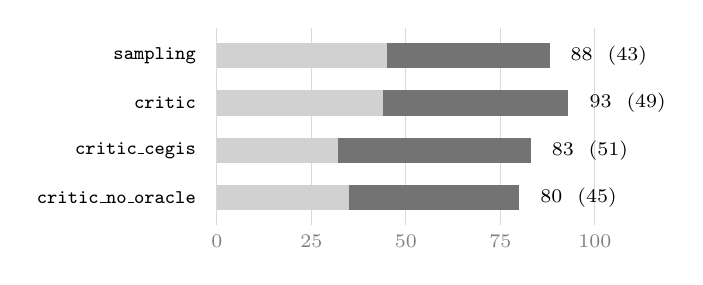
\begin{tikzpicture}[x=0.048cm, y=1cm]
  \def\yA{2.4} \def\yB{1.8} \def\yC{1.2} \def\yD{0.6}
  \draw[gray!50] (0,0.25) -- (0,2.75);
  \foreach \x in {0,25,50,75,100} {
    \draw[gray!30] (\x,0.25) -- (\x,2.75);
    \node[font=\scriptsize, gray, below] at (\x,0.25) {\x};
  }
  % segmento claro = 1a geração; escuro = ciclo. Lê \G* do painel.
  \fill[black!18] (0,\yA-0.16) rectangle (\GsampUm,\yA+0.16);
  \fill[black!55] (\GsampUm,\yA-0.16) rectangle (\GsampTot,\yA+0.16);
  \fill[black!18] (0,\yB-0.16) rectangle (\GcritUm,\yB+0.16);
  \fill[black!55] (\GcritUm,\yB-0.16) rectangle (\GcritTot,\yB+0.16);
  \fill[black!18] (0,\yC-0.16) rectangle (\GcegisUm,\yC+0.16);
  \fill[black!55] (\GcegisUm,\yC-0.16) rectangle (\GcegisTot,\yC+0.16);
  \fill[black!18] (0,\yD-0.16) rectangle (\GnoorUm,\yD+0.16);
  \fill[black!55] (\GnoorUm,\yD-0.16) rectangle (\GnoorTot,\yD+0.16);
  \node[font=\scriptsize, anchor=east] at (-3,\yA) {\texttt{sampling}};
  \node[font=\scriptsize, anchor=east] at (-3,\yB) {\texttt{critic}};
  \node[font=\scriptsize, anchor=east] at (-3,\yC) {\texttt{critic\_cegis}};
  \node[font=\scriptsize, anchor=east] at (-3,\yD) {\texttt{critic\_no\_oracle}};
  \node[font=\scriptsize, anchor=west] at (\GsampTot+3,\yA)  {\GsampTot{} \ (\GsampCiclo)};
  \node[font=\scriptsize, anchor=west] at (\GcritTot+3,\yB)  {\GcritTot{} \ (\GcritCiclo)};
  \node[font=\scriptsize, anchor=west] at (\GcegisTot+3,\yC) {\GcegisTot{} \ (\GcegisCiclo)};
  \node[font=\scriptsize, anchor=west] at (\GnoorTot+3,\yD)  {\GnoorTot{} \ (\GnoorCiclo)};
\end{tikzpicture}
\caption{Decomposição das vitórias, em tarefas resolvidas de \An{}. O segmento
claro são as decididas na primeira geração, comum às quatro condições; o escuro,
as atribuíveis ao ciclo. Os rótulos dão o total e, entre parênteses, a parcela do
ciclo. A ordenação pelo total (\GcritTot{}, \GsampTot{}, \GcegisTot{},
\GnoorTot{}) \emph{inverte} quando se olha apenas o ciclo (\GcegisCiclo{},
\GcritCiclo{}, \GnoorCiclo{}, \GsampCiclo{}): as três condições de crítico passam
à frente da linha de base.}
\label{fig:decomposicao}
\end{figure}

O resultado é que \vereditoDois{}. Restringindo cada par às tarefas que a
primeira geração não resolveu em nenhuma das duas condições, restam \Rn{} tarefas
— cerca de um quinto da amostra discrimina de fato — e todos os
\numComparacoes{} $p$-valores ficam entre \RpMenor{} e \RpMaior{}. O mesmo padrão
aparece numa medição anterior sobre as mesmas tarefas, com duas condições e um
protocolo de crítico diferente: descontada a primeira geração, o placar fica
empatado em \Bciclo{}\,$\times$\,\Bciclo{} sobre \BdiscrimN{} tarefas.

Duas leituras decorrem daí. A primeira é metodológica: o poder estatístico
efetivo de uma comparação entre arquiteturas de agentes é muito menor do que $n$
sugere. A segunda vai na direção oposta ao número bruto: descontada a primeira
geração, as três condições de crítico ficam \emph{acima} de \texttt{sampling} em
vitórias do ciclo (\GcegisCiclo{}, \GcritCiclo{} e \GnoorCiclo{} contra
\GsampCiclo{}). As diferenças são pequenas e nenhuma é significativa, mas a
direção depende de qual quantidade se observa — dependência invisível em qualquer
relato que reporte apenas acurácia agregada. O confundimento é eliminável por
construção: basta que a primeira condição a alcançar uma tarefa grave a primeira
geração e as demais a repitam, com a repetição ainda debitada do orçamento, o que
de quebra economiza \SeedEconomia{} chamadas em um bloco de quatro condições.

\section{Discussão}

A leitura defensável é pragmática: sob orçamento de chamadas igualado, alocar o
orçamento em diversidade não é distinguível de alocá-lo em revisão dirigida — nem
mesmo quando a revisão é guiada por um oráculo indisponível a qualquer sistema
autônomo. Como o desenho favorece a via iterativa por construção, o resultado é
mais informativo do que um empate entre esquemas equivalentes: indica que a
informação privilegiada, isoladamente, não é o fator limitante. Não sustenta,
porém, a leitura causal de que a assimetria de informação seja irrelevante — as
condições diferem em vários eixos, e os intervalos de confiança admitem efeitos
que a medição não teria poder para detectar.

O achado mais consequente é o outro, e ele não é específico deste arranjo:
qualquer comparação entre esquemas de inferência que partam do mesmo
\emph{prompt} inicial herda o confundimento da primeira geração, e nenhuma
métrica agregada o revela. Uma verificação por subamostragem sem reposição das
próprias \An{} tarefas (\SubRep{} repetições) mostra a consequência prática: com
\SubNa{} tarefas, a direção observada em \An{} se reproduz em apenas \SubDirA\%
das subamostras — indistinguível de um sorteio — e a ordenação completa das
quatro condições, em \SubOrdA\%; com \SubNb{} tarefas, em \SubOrdB\%. Estudos
desta classe conduzidos em algumas dezenas de tarefas não estão medindo direção
\citep{button:13}.

\paragraph{Limitações.} A dominante é o confundimento da primeira geração, que
reduz o $n$ efetivo e cuja correção, embora conhecida e barata, não foi aplicada
aqui. Seguem-se: o orçamento é medido em chamadas, não em tokens — as condições
de crítico consomem de \AtokExcessoMin\% a \AtokExcessoMax\% mais tokens por
tarefa, e sob orçamento em tokens o sinal poderia inverter; os oráculos não são
autônomos, de modo que \texttt{critic} e \texttt{critic\_cegis} medem a validação
por oposição como limite superior, não um método implantável; há uma execução por
tarefa, então parte da variação é ruído do modelo, mitigado pelo pareamento mas
não eliminado; \texttt{sampling} foi coletado em data anterior à das condições de
crítico, e o modelo é hospedado, o que introduz um confundimento temporal nas
comparações que envolvem a linha de base; e o filtro anti-vazamento captura grades
e código, mas não paráfrases, de modo que ele mede o que foi barrado, não o que
passou.

\section{Conclusão}

% >>> VEREDITO (conclusão)
Sob orçamento fixo de chamadas para síntese de programas no ARC-AGI-1, quatro
condições que variam isoladamente o acesso ao oráculo e a forma do feedback não
se separam em \An{} tarefas: \vereditoUm{}. O crítico opera como mecanismo,
atingindo a mesma consistência com os pares de demonstração com
\AreducaoProg\% menos programas, sem que isso se converta em acerto no teste.

O resultado mais transferível independe de qual condição venha a prevalecer:
\vereditoDois{}. Descontada essa parcela, a medição discrimina em cerca de um
quinto da amostra e a ordenação entre as condições inverte. O passo seguinte não
é aumentar $n$, e sim eliminar esse confundimento por construção e medir o
orçamento em tokens, que é a unidade de custo efetiva.

\section*{Reprodutibilidade}

Cada rodada grava um manifesto com a lista literal de identificadores de tarefa,
a semente, o orçamento e os modelos, além de um registro por condição com todos
os \emph{prompts}, respostas brutas, códigos gerados e resultados de execução. As
respostas brutas do Crítico são preservadas antes do filtro anti-vazamento, o que
permite auditar independentemente o que foi redigido e o que passou. Os testes
automatizados travam as propriedades críticas do desenho, incluindo a separação
de informação entre os \emph{prompts} do Gerador e do Crítico e a paridade de
orçamento entre as condições.

\bibliography{artigo}

\end{document}
